\documentclass{report}
\usepackage{ctex}
\usepackage{geometry}
\usepackage{graphicx}
\geometry{left=2.0cm, right=2.0cm, top=2.0cm, bottom=2.0cm}

\begin{document}

\begin{center}
    \fontsize{30}{0}西安交通大学城市学院\\
\fontsize{20}{0}\underline{多媒体技术及应用}实验报告
\end{center}

\noindent
\LARGE 班级 \underline{软件191} 姓名 \underline{胡瑞平} 学号 \underline{19031198} 专业 \underline{软件工程}\\
\LARGE 实验日期 \underline{2021} 年 \underline{11} 月 \underline{03} 日\\
审阅教师 \underline{\,\,\,\,\,\,\,\,\,\,\,\,\,\,\,\,\,\,\,\,\,\,\,\,\,}\\
实验名称 \underline{多媒体软件综合训练} 实验地点 \underline{行政楼203}\\

\noindent
\begin{tabular}{|p{18cm}|}
    \hline
    实验任务概要\\
    \\图形图像处理
    \\
    \\
    \\
    \\
    \hline
    学生实验心得及建议\\
    \\本次实验整体还算顺利,再接再厉!
    \\
    \\
    \\
    \\
    \hline
    教师批阅记录\\
    \\
    \\
    \\
    \\
    \hline
\end{tabular}

\newpage

\section*{\Huge 作品步骤}

1. 准备素材

\begin{figure}[!htbp]
    \centering
    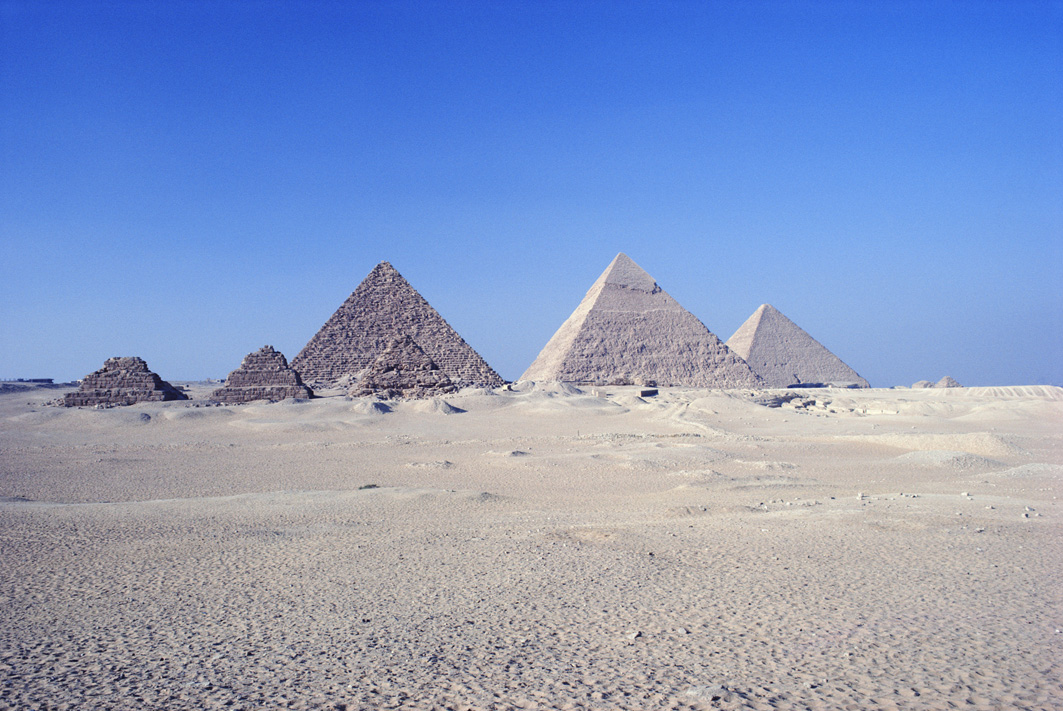
\includegraphics{2_1金字塔.jpg}
    \caption{素材1}
\end{figure}
\clearpage

\begin{figure}[!htbp]
    \centering
    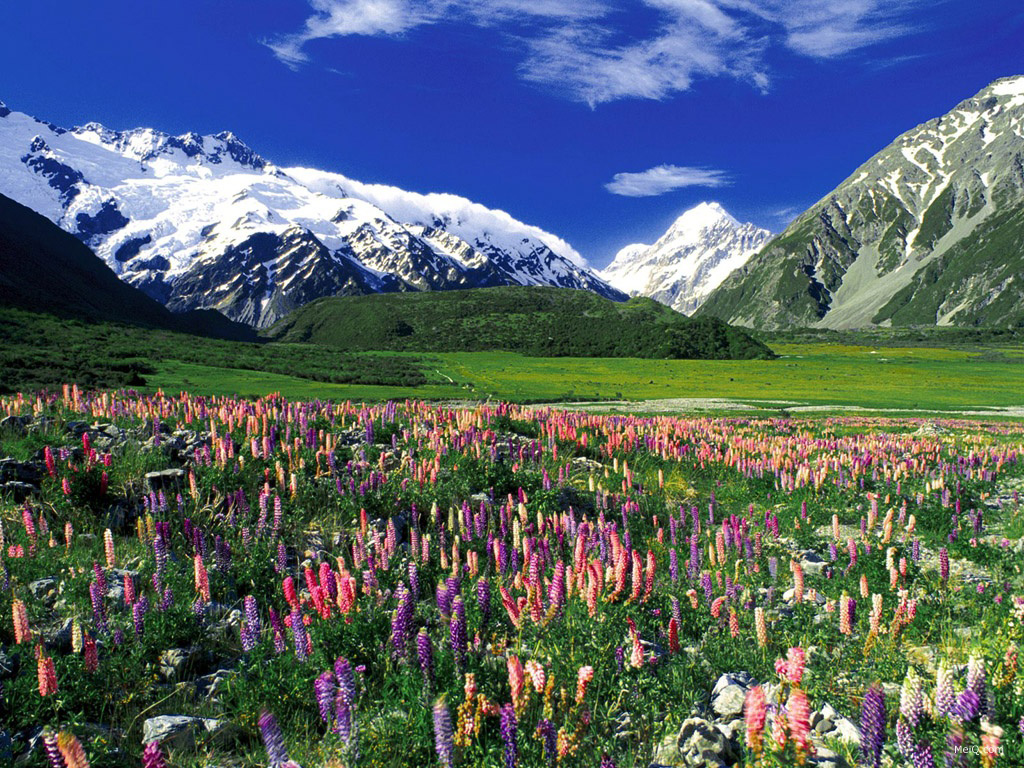
\includegraphics[scale=0.5]{2_2雪山绿地.jpg}
    \caption{素材2}
\end{figure}
\clearpage

2. 使用Photoshop分别将将素材1和素材2打开

\begin{figure}[!htbp]
    \centering
    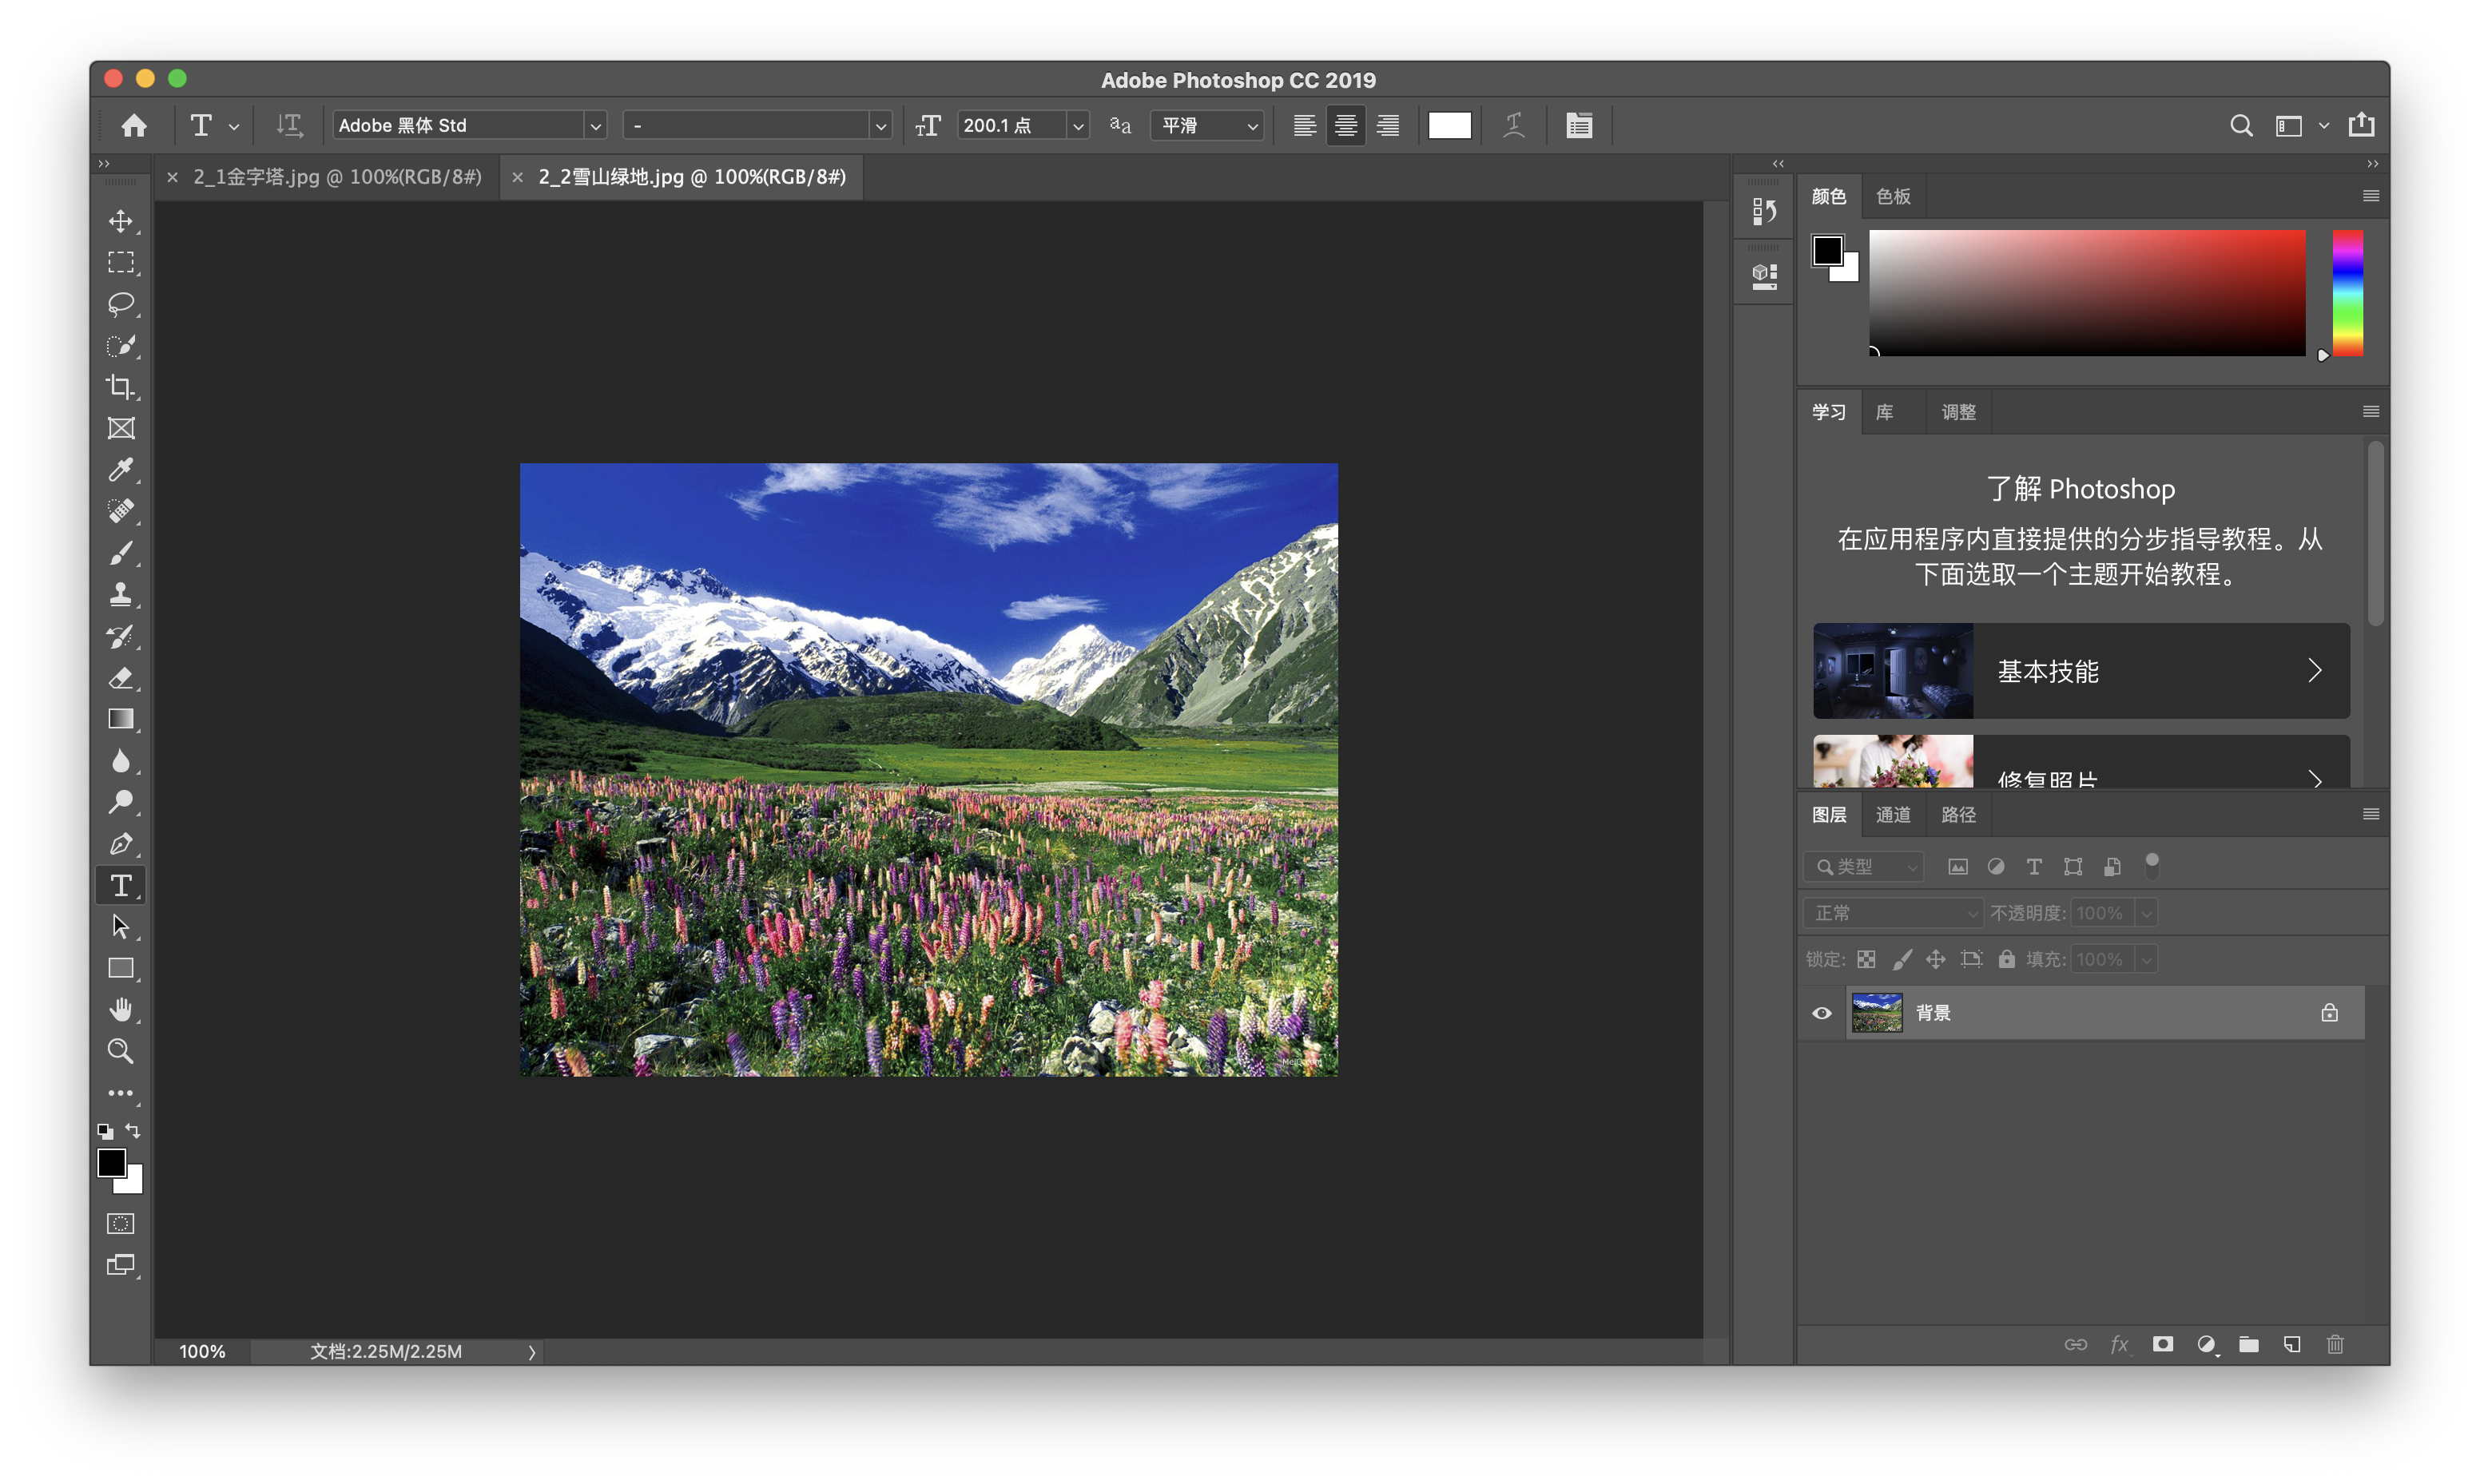
\includegraphics[scale=0.25]{截屏2021-11-09 下午9.28.38.png}
\end{figure}

3. 使用矩形选框工具大致框选素材二中的草地部分

4. 使用移动工具拖入素材1,使用自由变换命令大致覆盖素材1金字塔的地面部分

5. 使用橡皮擦工具,调至合适半径和力度,擦除多余部分

\newpage
6. 最终效果如图所示

\begin{figure}[!htbp]
    \centering
    \includegraphics[scale=0.35]{截屏2021-11-09 下午9.36.34.png}
\end{figure}

\end{document}